\section{Planar Graph Sparsity}

\begin{frame}
\frametitle{\secname}

\begin{columns}
\column{0.6\textwidth}
\begin{wideitemize}
\item<1-> Simple graphs have $O(n^2)$ edges
\item<1-> Planar graphs have $\le3n-6=\emph{O(n)}$ edges!\footnote{Assuming faces have degree $\ge3$}
\item<1-> Fursuits are planar graphs
\item<1-> $\text{Seam count}=O(\text{Fabric patch count})$

\item<2-> Each patch you add only introduces a constant number of new seams you have to sew!
\item<3-> Therefore, it is totally reasonable to have 64 patches for your fursuit /j
\end{wideitemize}

\column{0.05\textwidth}


\column{0.35\textwidth}
    \only<2>
    {
    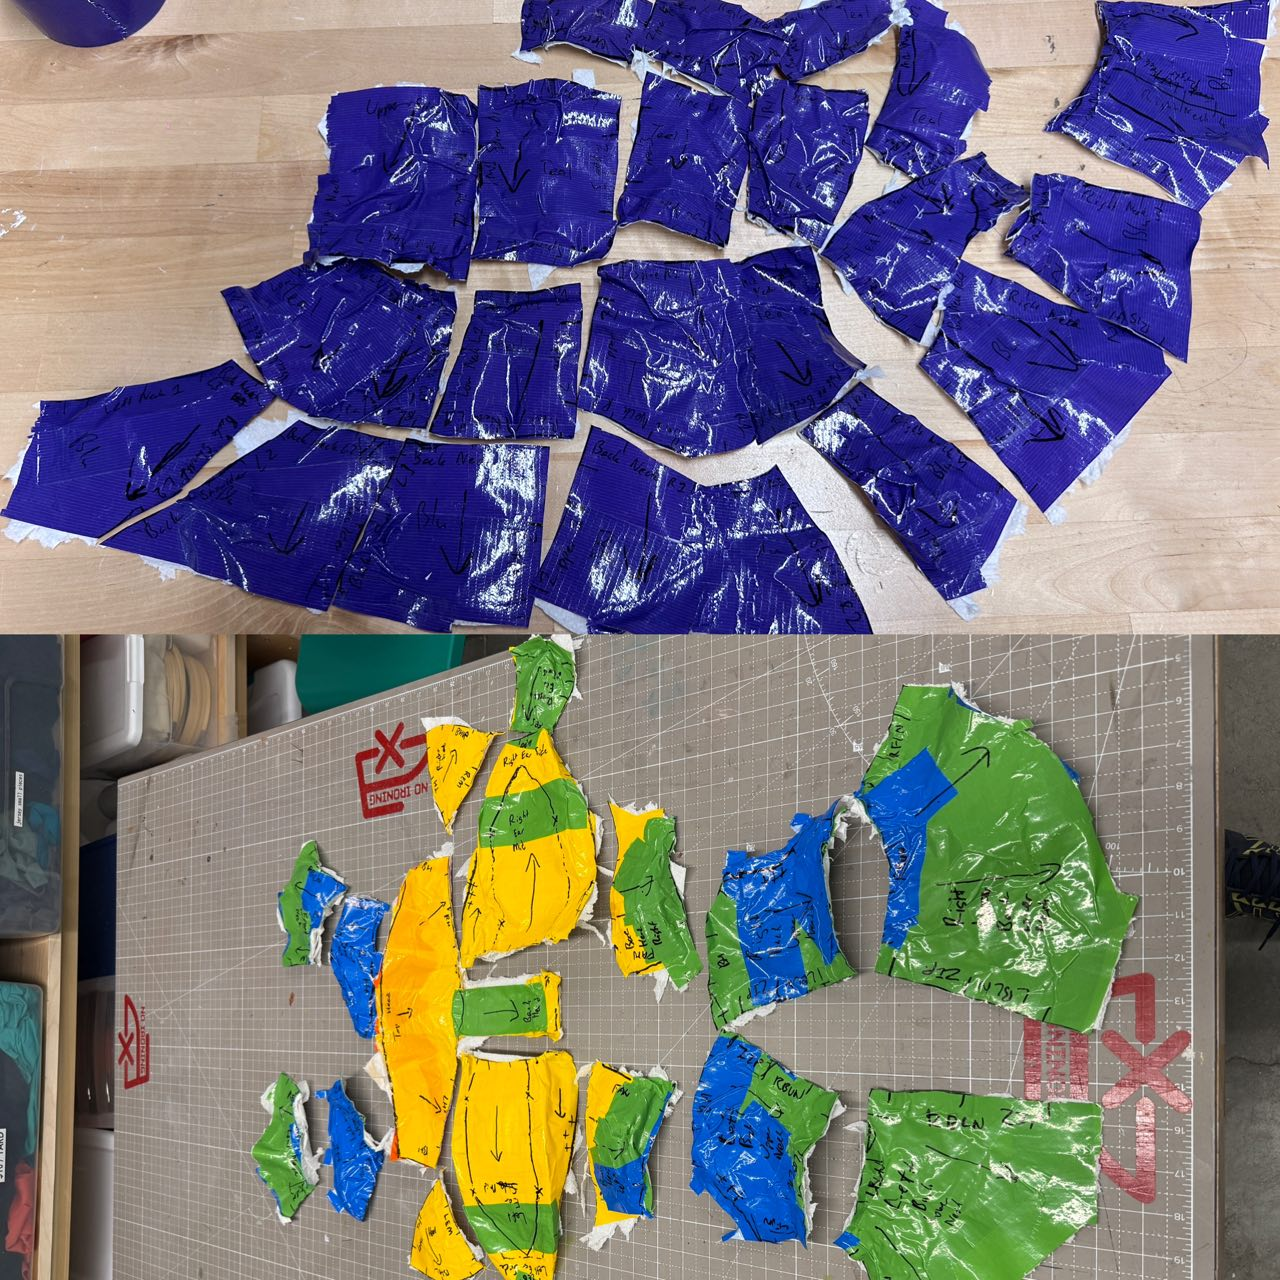
\includegraphics[width=1\linewidth]{slides//planar_fursuit/planar_fursuit_bunsen_comparison.png}
    
    {
    \tiny
    Top: Bunsen's V1 pattern with 40 pieces total (not all shown)

    Bottom: Bunsen's V2 pattern with 19 pieces total
    }
    }
    \only<3->
    {
    \includegraphics[width=\textwidth,angle=180,origin=rb]{slides/planar_fursuit/long_body_assembled.jpg}
    {
    \tiny
    A part of Long's pattern with \char`~16 pieces
    }
    }
\end{columns}

\end{frame}
